\section{Постановка задачи}
\label{sec:theory}

% Расскажем об импульсных динамических системах подробнее и подведем %
% соотв. теоретическую базу.
%\section {Импульсные управления}
\subsection {Уравнение эйконала}
\label{sec:csdisttrack}


Предположим, что у нас есть некоторая замкнутая кривая $l$,
разделяющая $\mathbb{R}^2$ на внутреннюю область$\Omega$ и
внешнюю. Пусть $l$ задает фронт волны. Предположим, что волна движется
с известной скоростью $F$, как показано на
рисунке~\ref{fig:eikvis}. Для наших потребностей достаточно
предположить, что кривая расширяется, т.е. ее движение направлено
вовне текущей области $(F>0)$, а также игнорируется касательная
компонента движения, т.е. волна распространяется только по
нормали к кривой.

\begin{figure}[h]
  \centering
  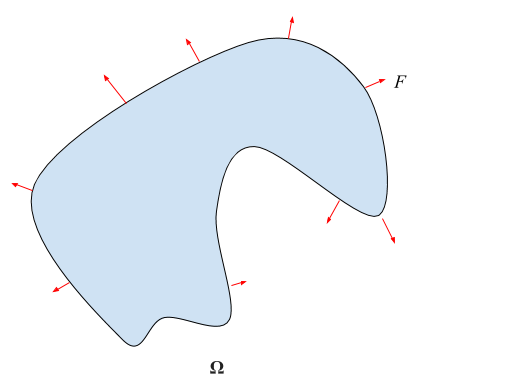
\includegraphics[width=0.5\linewidth]{img/eikonal_vision.png}
  \hfil \caption{распространение кривой со скоростью $F$}
  \label{fig:eikvis}
\end{figure}


Для того, чтобы определить положение волнового фронта в каждый момент
времени, мы можем вычислить время прибытия $T$, когда впервые будет
пересечена точка $(x,y)$.

Если взять одномерный случай, то там мы можем вычислять расстояние как
произведение скорости на время, тогда мы можем записать уравнение для
функции $T$:

\begin{equation*}
  1 = F \frac{dT}{dx}
\end{equation*}

В пространствах более высокой размерности время прибытия T это решение
задачи Дирихле для уравнения эйконала.

\begin{equation}
  \label{eq:eikonal}
  \left\{ \begin{matrix}
      F(x) \| \nabla T(x) \| = 1, x \in \Omega \\
      T(x) = 0, x \in \Gamma
    \end{matrix}\right.
\end{equation}

Здесь $\Omega$ -- это область в $\mathbb{R}^2$, $\Gamma$ -- начальная
состояние кривой, $\nabla$ обозначает градиент, и $\| \cdot \|$ является
евклидовой нормой.

Стоит отметить, что эволюция кривой содержит больше информации чем
время первого прибытия: фронт может проходить через одну и ту же точку
несколько раз. Для иллюстрации рассмотрим распространение
волнового фронта со скоростью $F \equiv 1$, как представлено на
рисунке~\ref{fig:prpgt-eik}

\begin{figure}[h]
  \centering
  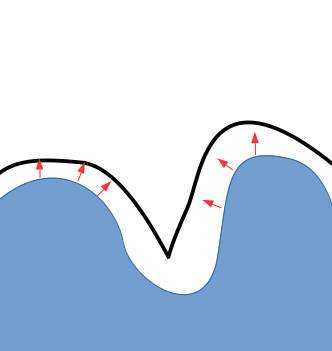
\includegraphics[width=0.3\linewidth]{img/propagate_eikonal.png}
  \hfil \caption{распространение кривой со скоростью $F \equiv 1$}
  \label{fig:prpgt-eik}

\end{figure}

Жирная линия указывает где будет кривая на следующем шаге.
Предположим, теперь мы хотим заглянуть дальше. Тогда мы получим
следующую картину на рисунке~\ref{fig:swallow-ex} кривая пройдет
сквозь себя, образовав так называемый \textit{ласточкин хвост}. Чем он
плох? Мы в некоторых точках получаем многозначную функцию, чего нужно
избегать. В \cite{S1999}, Сетиан описывает эту ситуацию, как если мы
рассмотрим фронт распространения кривой, как фронт распространения
огня, тогда то, что было однажды сожжено, второй раз не сжигается.
Следовательно, нам стоит выбрать в каком-то смысле физически
корректное решение как на рисунке~\ref{fig:correct-exmp}

\begin{figure}[h]
  \centering
  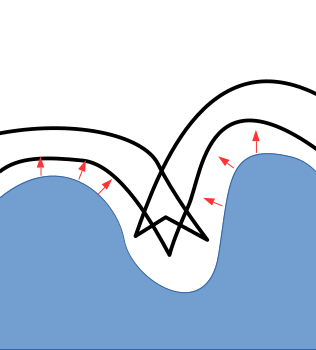
\includegraphics[width=0.3\linewidth]{img/swallow-tail-example.png}
  \hfil \caption{Пример ласточкиного хвоста}
  \label{fig:swallow-ex}

\end{figure}

\begin{figure}[h]
  \centering
  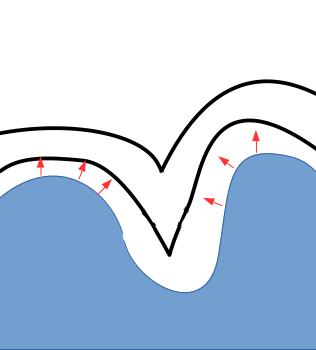
\includegraphics[width=0.3\linewidth]{img/corrct-example.png}
  \hfil \caption{Пример корректного решения}
  \label{fig:correct-exmp}

\end{figure}

Уравнение~\eqref{eq:eikonal} является частным случаем \textit{уравнения
Гамильтона-Якоби} первого порядка, которое в стационарном случае выглядит
следующим образом:

\begin{equation}
  \label{eq:hje}
  \left\{ \begin{matrix}
      H(x, \nabla T(x)) = 0,\text{на } \mathbb{R}^n \times (0,\infty) \\
      T(x) = 0,  \text{на } \mathbb{R}^n \times \{t = 0\},
    \end{matrix}\right.
\end{equation}
где гамильтониан $H = H(x,\nabla T(x))$ непрерывная вещественная функция на
$\mathbb{R}^n \times \mathbb{R}^n$ и $\phi : \mathbb{R}^n \rightarrow
\mathbb{R}$ -- начальные условия.

Если $H(x,p) = |p| H(x,p/|p|) = |p| F(x)$, тогда мы получаем
обыкновенное уравнение эйконала для изотропного случая
\eqref{eq:eikonal}, если гамильтониан имеет вид
$H(x,p) = \|p\| F(x, \frac{p}{\|p\|})$, тогда мы имеем анизотропное
уравнение эйконала.

Если $H(x,p) = |p| H(x,p/|p|) = |p| F(x)$, тогда мы получаем
обыкновенное уравнение эйконала для изотропного случая
\eqref{eq:eikonal}, в противном случае уравнение будет анизотропным

В общем случае это уравнение не имеет классических $C^1$
решений. Проблема эта имеет решение в обобщенных решениях, которые
непрерывны и удовлетворяют данному уравнению в частных производных
почти всюду. Использование вязкостных  решений, предложенных в
\cite{V1984,V1983} для задач первого порядка позволяет выбрать одно
``физическое'' решение из множества других. 

\subsection{Вязкостные решения}

В качестве примера давайте рассмотрим следующую задачу

\begin{equation}
  \label{eq:visc_sample}
  \left\{ \begin{matrix}
      |T'(x)| = 1,\text{на } (-1,1) \\
      T(x) = 0,x = \pm 1
    \end{matrix}\right.
\end{equation}

Здесь мы видим одномерное уравнение эйконала. Общим решением такого
уравнения будет $T(x) = \pm x + c$, но мы не можем выбрать знак $x$ и
константу для того, чтобы удовлетворить граничным условиям. Вместо
этого есть слабое решение, которое удовлетворяет дифференциальному
уравнению почти всюду.

Функция:
\begin{equation*}
  T(x) = 1 - |x|
\end{equation*}
удовлетворяет граничному условию и дифференциальному уравнению почти
всюду, за исключением точки $x = 0$. Это решение дает расстояние до
границы области, но не является единственным. Как показано на
Рисунке~\ref{fig:weak-sol}, существует бесконечно много функций,
удовлетворяющих граничным условиям почти всюду.

\begin{figure}[h]
  \centering
  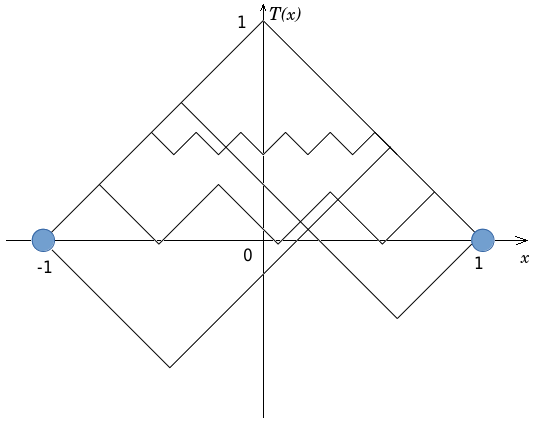
\includegraphics[width=0.5\linewidth]{img/weak-sol.png}
  \hfil \caption{слабые решение $|T'|=1,T(-1)=T(1)=0$}
  \label{fig:weak-sol}

\end{figure}

Если мы добавим к уравнению \eqref{eq:visc_sample} слагаемое,
отвечающее за вязкость, то получим уравнение 2-го порядка для
$T_\epsilon(T)$:

\begin{equation}
  \label{eq:visc_sample_2}
  \left\{ \begin{matrix}
      -\epsilon T''_\epsilon+|T'(x)| = 1,\text{на } (-1,1) \\
      T_\epsilon(-1) = T_\epsilon(1) = 0.
    \end{matrix}\right.
\end{equation}

Уравнение \eqref{eq:visc_sample_2} имеет единственное решение:

\begin{equation*}
  T_\epsilon(x) = 1 - |x| + \epsilon e^{-1/\epsilon}(1 - e^{(1-|x|)/\epsilon})
\end{equation*}


На рисунке~\ref{fig:viscosity-experiment} изображены решения уравнения
\eqref{eq:visc_sample_2} для  $\epsilon =
1/5,1/10,1/20,1/40,1/100$. Для малых $\epsilon$, вязкостный член
сглаживает часть решения $T_\epsilon(x)$. Фактически он сглаживает
углы и делает решение $C^2$ гладким. В этом примере мы выбрали
$\epsilon >0$ для того, чтобы сгладить решение около локальных максимумов, выбором
$\epsilon <0$ можно получить решения аппроксимирующие $T(x) = |x| -
1$,которые сглаживают его относительно локальных минимумов. При
стремлении $\epsilon$ к нулю, $T_\epsilon$ сходится к вязкостному
решению \eqref{eq:visc_sample}. Подробнее об этом можно прочесть в
работах \cite{V1984,V1983}.


\begin{figure}[h]
  \centering
  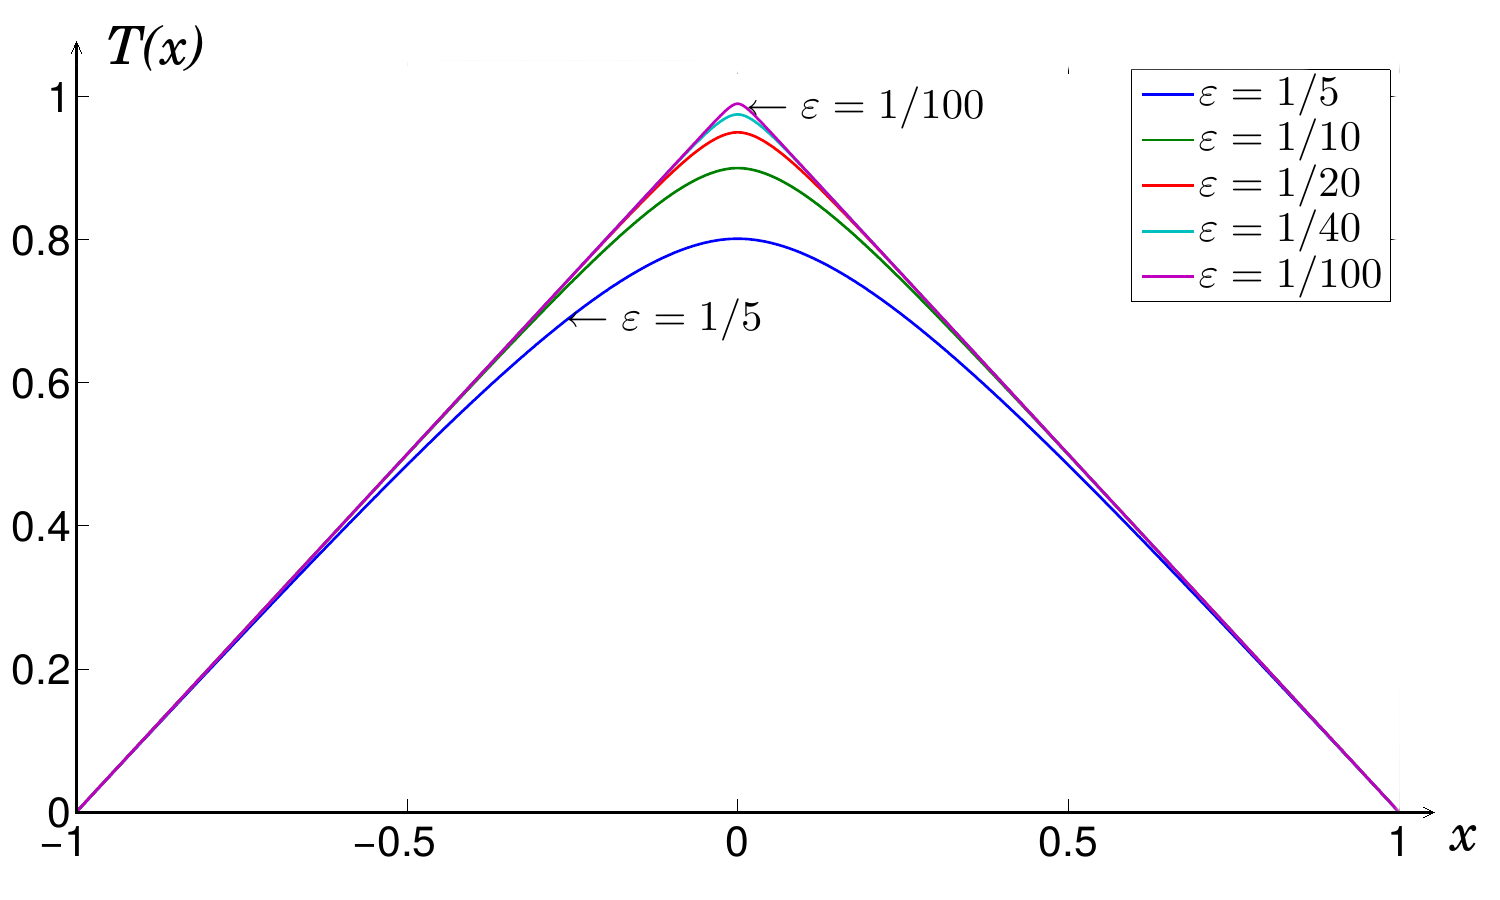
\includegraphics[width=\linewidth]{img/viscosity_example.png}
  \hfil \caption{Решение уравнения \eqref{eq:visc_sample_2} для $\epsilon = 1/5, 1/10, 1/20, 1/40, 1/100$}
  \label{fig:viscosity-experiment}

\end{figure}


% \subsection{Анизотропное уравнение эйконала}

% Предположения, которые выдвигались вначале обзора касались изотропного
% случая, когда на скорость распространения кривой не влияло ее текущее
% местоположение. Мы расширим наше уравнение Гамильтона-Якоби


%%% Local Variables:
%%% mode: latex
%%% TeX-master: "eikonal_solver"
%%% End:
